\subsection{Træning}
Efter brugeren har angivet sin daglige helbredstilstand starter træningen. Før selve træningen kan påbegyndes, spørger systemet brugeren om, hvorvidt kompatible enheder skal tilkobles. Dette kan eksempelvis være en pulsmåler. Vælger brugeren ikke at tilkoble eksterne enheder, startes tiden og GPS, hvorefter selve træningen påbegyndes. Vælger brugeren at tilkoble enheder, prøver systemet at synkronisere med enhederne.  Hvis dette lykkes, påbegyndes selve træningen og alle måleenhederne starter.

Under træningen kan brugeren pause træningen og måleenhederne, hvorefter der er mulighed for at fortsætte træningen eller afslutte træningen. Afsluttes træningen, vises app'ens hovedmenu og træningen er dermed ikke fuldført. 
Hvis træningen fuldføres, skal brugeres evaluere træningen fra et til fem. Herefter vises resultater fra den udførte træning. Systemet sender den daglige helbredstilstand, resultater fra den udførte træning samt evaluering til databasen, som lagrer informationerne. 
Af \autoref{fig:traening} fremgår aktivitetsdiagram over træning.

\begin{figure} [H]
\centering
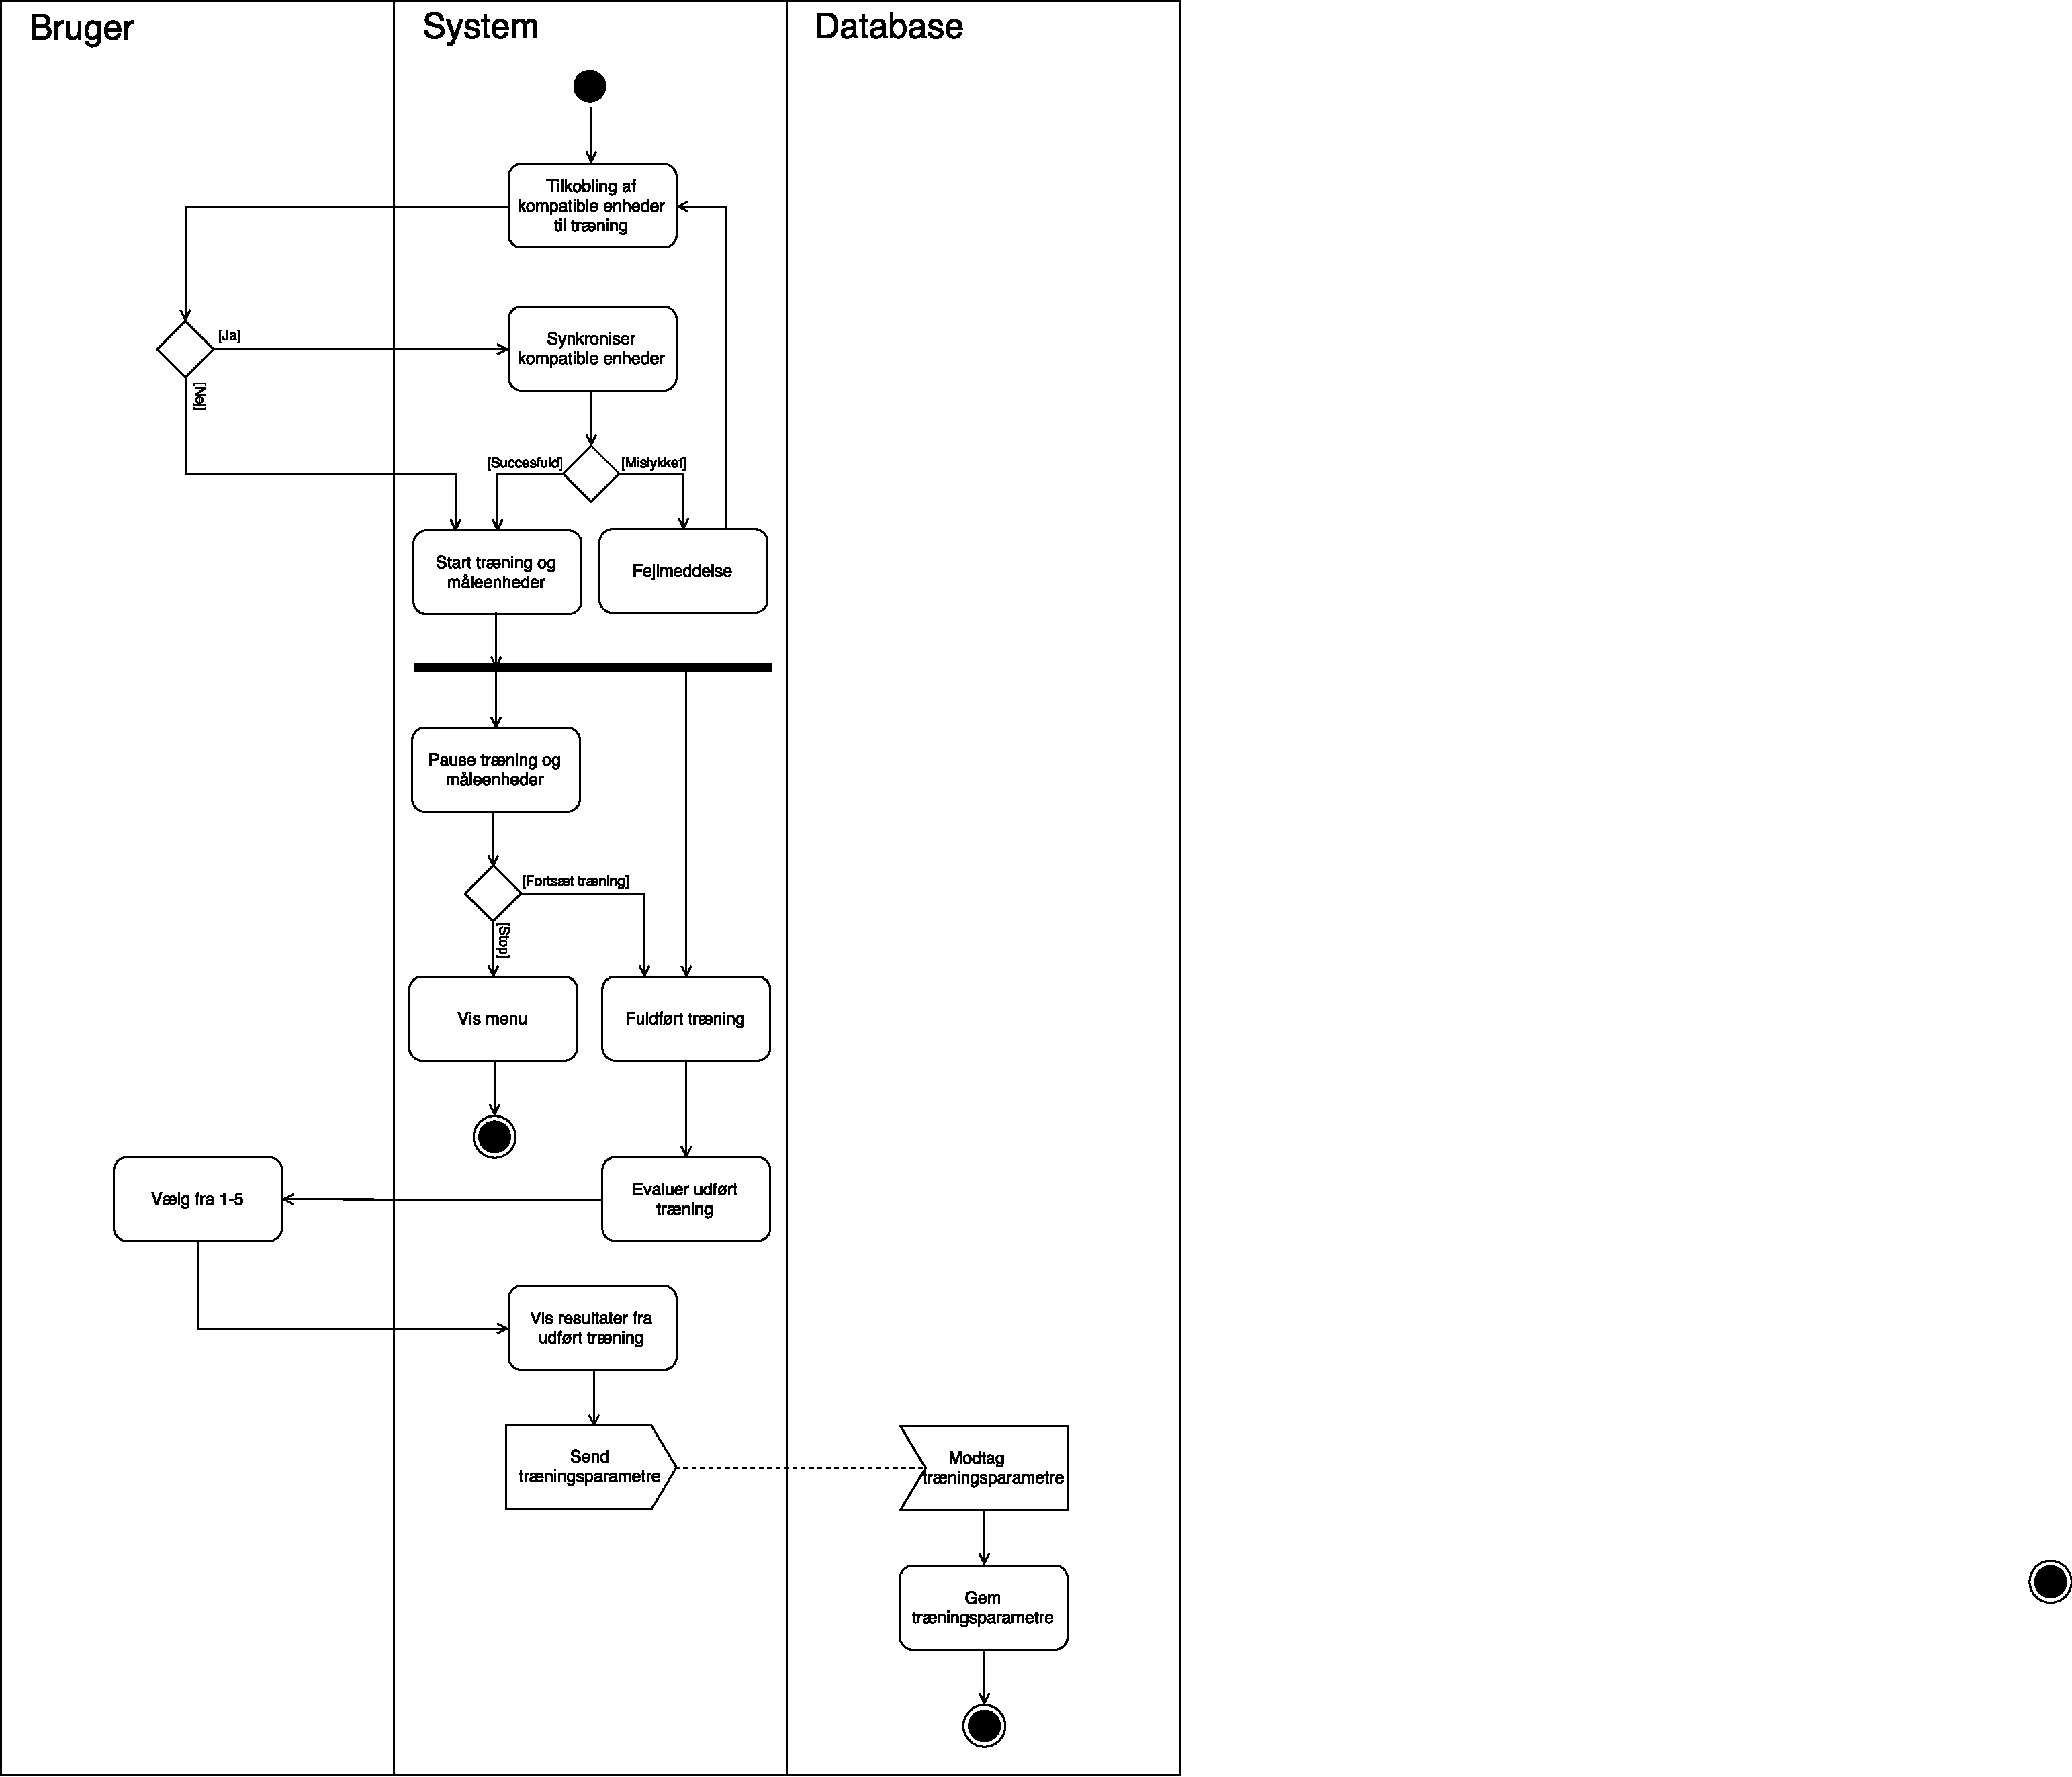
\includegraphics[width=0.9\textwidth]{figures/aktivitetsdiagram/Traening}
\caption{Aktivitetsdiagram over træning.}
\label{fig:traening}
\end{figure}
